%Replace Strings:
%PROJECT.TITLE
%TODO.CHANGE
%PROJECT.ABSTRACT.KEYWORDS

\documentclass[12pt, a4paper, oneside]{article}

\usepackage[utf8]{inputenc}
\usepackage[bindingoffset=1.57cm, left=2.54cm, right=2.54cm, top=2.54cm, bottom=2.54cm]{geometry}
\usepackage{mathptmx}
\usepackage{fancyhdr}
\usepackage{lipsum}
\usepackage{secdot}
\usepackage{lastpage}
\usepackage{cite}

\usepackage{graphicx}
	\graphicspath{ {images/} }

\usepackage{tocloft}
\usepackage[table,xcdraw]{xcolor}

\usepackage{floatrow}
\floatsetup[table]{capposition=top}

\linespread{1.2}
\pagestyle{fancy}
\fancyhf{} % sets both header and footer to nothing
\renewcommand{\headrulewidth}{0pt}
\rhead{ \textit{TreasureNepal2020: Discover Places, Collect Treasures}}
\cfoot{\thepage}

\setlength{\parindent}{0pt}
\setlength{\parskip}{12pt}

%\frontmatter

\begin{document}

\pagenumbering{roman}
\addcontentsline{toc}{section}{Abstract}
\large
\begin{center}
	\textbf{ABSTRACT}
\end{center}

\normalsize
As we are at the brim of the Visit Nepal year 2020, the decentralization of tourism in Nepal has become absolutely necessary. Almost ninety percent of the tourists arriving Nepal visit the most popular destinations like Kathmandu, Pokhara, Chitwan and Everest, whereas the remote places like Rara Lake and Phoksundo National Park have not seen satisfactory inflow of tourists despite them being rich in natural beauty and tourism potentiality. There are still a lot of tourist destinations in Nepal that need the attention of the tourists.

TreasureNepal2020 is a treasure hunt application where the users travel to different places in order to collect treasures and increase their scores. The project aims to take the attention of tourists and visitors towards various tourists destinations in Nepal. The tourists need to physically reach to a place in order to collect treasures. The tourists who collect treasures at places that are remote and left behind will get higher scores than the ones who visit common popular destinations. The users can also share their scores and leaderboard status to social media. On the long run, the project sets its objective to take the tourism of Nepal to a new level.

The major deliverables proposed in the project are an Android application and a RESTful API web service.

\textbf{Keywords}: Visit Nepal 2020, Treasure hunt, Tourism\\

\break

\large
\begin{center}
	\textbf{TABLE OF CONTENTS}
\end{center}


\normalsize
\setlength{\cftbeforetoctitleskip}{0pt}
\renewcommand{\contentsname}{}
\tableofcontents

\break

%\mainmatter
\cfoot{\textbf{\thepage} /  \pageref{LastPage}}

\pagenumbering{arabic}
\section{Introduction} 
TreasureNepal2020 is a mobile application for a treasure hunt game proposed to be tailored for tourists visiting Nepal in the year 2020. With the view of encouraging tourists to visit remote and unexplored part of the country, the application aims to increase the traffic of tourist in such locations as well as promote their tourism. This document looks forward to providing essential information about the needs, scope, objectives and proposed methodology of the application.

\subsection{Problem Statement}
Tourism has a great potential to contribute to the Gross Domestic Product (GDP) of Nepal, but having observations at the statistics, the ratio of contribution of tourism to GDP is not satisfactory. According to Nepal Rastra Bank, the total conbtribution of the foreign exchange from tourism to the total Gross Domestic Product (GDP) of Nepal was 2.2\% in the year 2017/18. \cite{tourismstats}.

Tourism in Nepal is largely centralized to a few popular destinations. The places like Kathmandu, Pokhara, Chitwan, Annapurna area and Everest area are largely flocked by tourists while destinations like Rara Lake, Shey Phoksundo National Park or Khaptad National park struggle to get satisfactory inflow of traffic. This decentralisation of tourism has largely underestimated the potential and beauty of many travel destinations, specially in remote areas. In addition, as majority of people in such places rely solely on tourism industry for their livelihood, this problem has pushed those communities even further down below the poverty line.

The Government of Nepal has taken efforts to celebrate the year 2020 officially as the Visit Nepal Year 2020. At the brim of year 2020, the authors have proposed to build a treasure hunt application specially tailored for the tourists to get their attention to unexplored and remote tourism destinations of Nepal.

\subsection{Project Objectives}
The proposed project has put forward the following objectives:

\begin{itemize}
	\item To decentralize the tourism industry and encourage uniform flow of tourists at various destinations across Nepal.
	\item To promote and encourage the tourism in remote and novel destinations which otherwise are not popular or have low inflow of tourists.
	\item To explore business and economic opportunities generated by the project if taken to the production level.
\end{itemize}

\subsection{Significance of the Study}
The project proposed is significant owing to the fact that we are near the Visit Nepal Year 2020, and the proposed project will certainly be fruitful in achieving the objectives set by the Government of Nepal in the year 2020. Since the proposed idea is one of the first of its kind, it is expected that the project will reach to a significant majority of tourists that visit Nepal in 2020.

\subsection{Scope and Limitations}
In the beginning phase, the treasure hunt concept of the app will be implemented and other features are proposed to be added later gradually if possible. Such possible extensions could be addition of forex plugins, itinerary maps, guides, etc. The users will be able to collect coins from collecting the treasures, and their collection will be put in the leaderboards based on the user's local location as well as country-wise and globally. The application will also be connected to third party social networking platforms like Facebook, Twitter, etc. so that the users can share their collection and score. 

The scores of the treasures will be calculated based on the factors like the difficulty to reach the destination, its novelty, potentiality to attract new tourists and other similar criteria. The users will receive more amount of score when visiting rural and novel places than visiting urban and frequently visited places.

The following are the limitations of the project that are realized:
\begin{itemize}
 	\item The application will be built on Android platform in the beginning and later extended to iOS, but not for other mobile operating systems like Blackberry and Windows.
	\item QR code scanning will be the method of collection of treasures and no other validation architecture will be used except for the check of location when the user scans the QR.
 \end{itemize}

%\break
%\section{Literature Review}
%This section consists description of the literature study performed during the development of this proposal.
%
%There are several treasure hunt applications available in the application stores developed for entertainment purposes. Some of them are GooseChase, Locandy, Huntzz, Scavify and Geocaching \cite{similarapps}.

\break
\section{Proposed Methodology}
This section describes the methodology that is proposed to be followed during the development of the project.

\subsection{Proposed Software Development Life Cycle}
The project will be developed as per the waterfall model of software development life cycle. The reason for choosing this model is the lack of sufficient time duration for agile and iterative methods, as well as very low chances of the changes of requirements in the process of development. The team will gradually move through the planning, requirements analysis, design, implementation. testing and deployment phases in a linear manner. However, there might be slight modifications in the original waterfall model where the design and implementation may be changed slightly after the testing phase if seen reasonable.

\subsection{Technical Architecture}
The application will be built upon the client-server web architecture, as illustrated in Figure \ref{fig:arch}.

\begin{figure}[h]
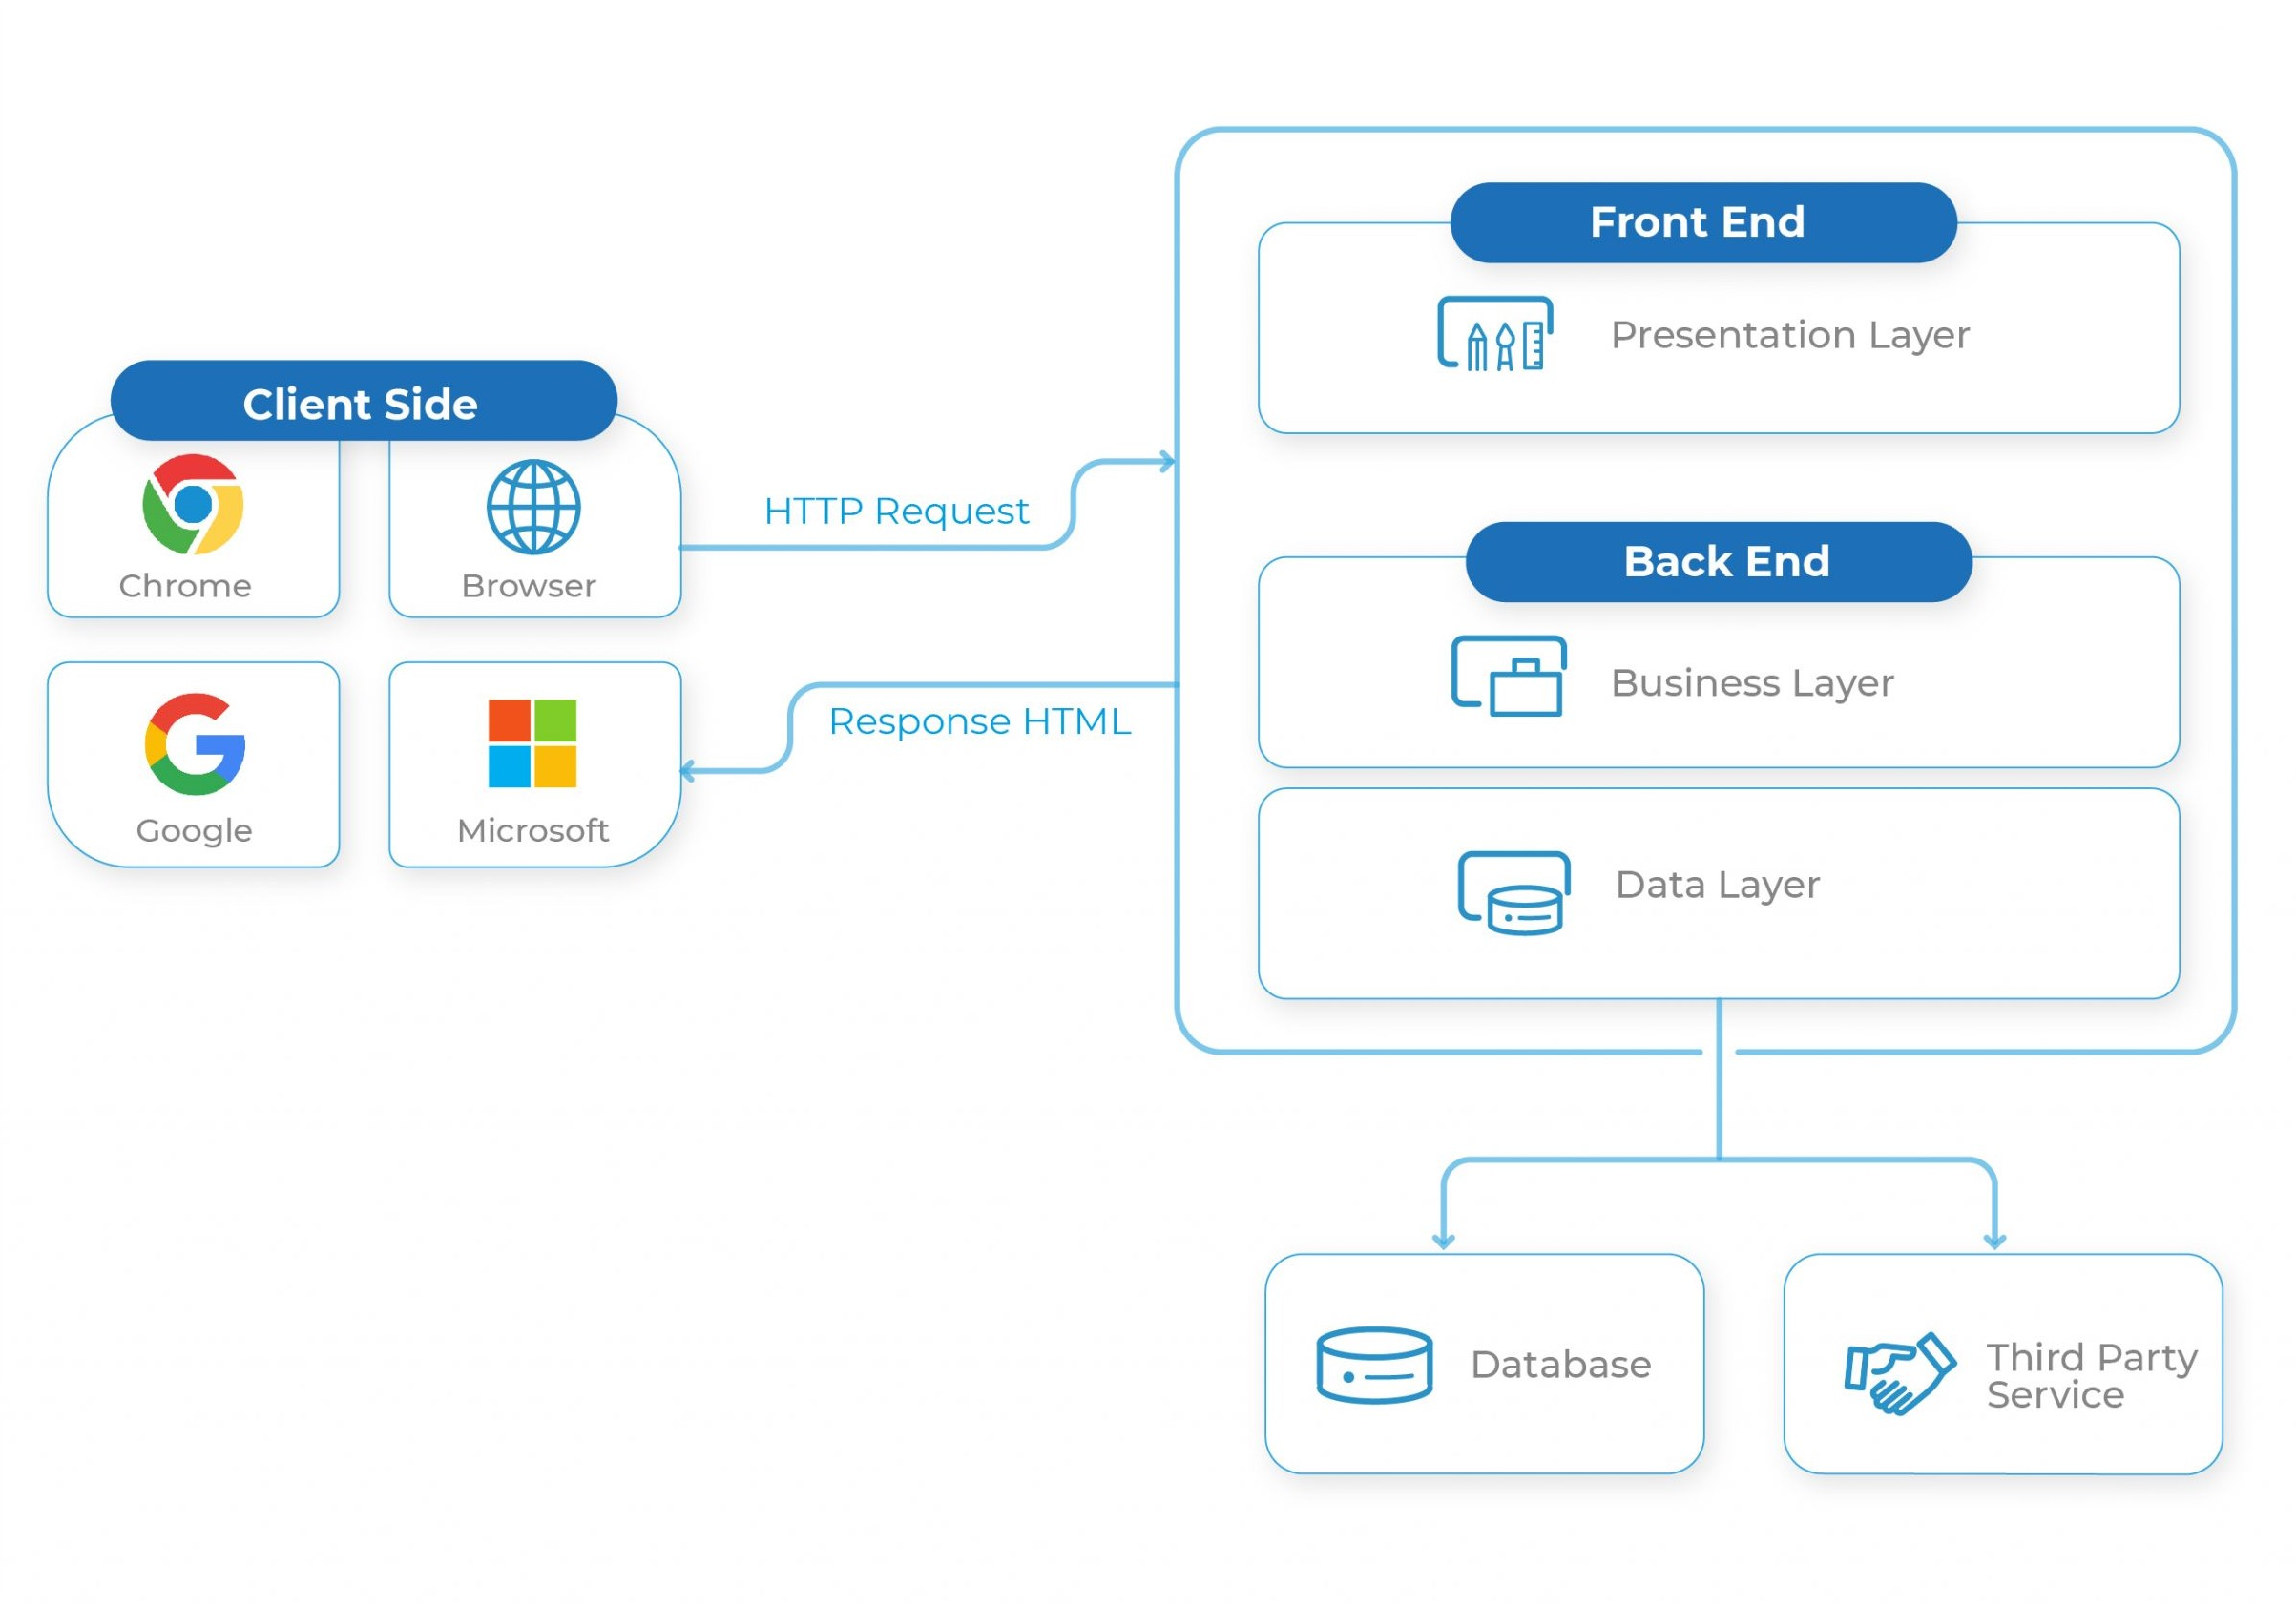
\includegraphics[width=\linewidth]{architecture}
\centering
\caption{Proposed architecture of the application}
\label{fig:arch}
\end{figure}

At the heart of the architecture lies the RESTful web service which communicates directly with the central database where all the data is stored. The mobile applications as well as the admin web interface do not access the database directly, but via the API service. The clients send HTTP requests like GET, POST and DELETE, while the API service processes those requests and return the data in JSON format.

\subsection{Proposed Technologies}
Table \ref{table:tech} consists of the major technologies that are proposed to be used during development and deployment of the application.

\renewcommand{\arraystretch}{1.5}
\begin{table}[h!]
\centering
\begin{tabular}{|l|l|}
\hline
\rowcolor[HTML]{C0C0C0} 
\textbf{Subject}    & \textbf{Proposed Technology} \\ \hline
Database            & MySQL                        \\ \hline
REST API Service    & Django REST Framework        \\ \hline
Android/iOS Client  & React Native                 \\ \hline
Admin Web Interface & Django Framework             \\ \hline
Deployment Platform & Amazon Web Services (AWS)    \\ \hline
Documentation & LaTeX \\ \hline
\end{tabular}
\caption{Technologies proposed to be used}
\label{table:tech}
\end{table}

\break
\section{Proposed Performance Analysis Methodology}
The performance analysis of the deliverables will be performed according to the popular Top Down Methodology. The main idea in this method is to analyse and address the higher order performance issues at first, then follow the lead upto the lower levels of details if needed \cite{tdmethod}. This methodology is proposed to be followed because it largely reduces the time and cost of assessing the performance since not every modules and sections of the project need to be analyzed at a deeper level.

The final evaluation of the project will be performed by the project evaluation team designated by the college administration.

\newpage
\newpage
\section{Proposed Deliverables}
The following will be the major deliverables that will be produced at the end of this project.

\subsection{RESTful API service}
There will be a running instance of RESTful API service developed and deployed at the end of the project. This API will be responsible for communicating between the client applications and the central database server.

\subsection{Android client application}
The application will be developed integrating all the features proposed earlier. The users will be able to use the application to scan QR codes at different travel destinations which will reward them with scores in their accounts. The application will also be integrated with social networking platforms like Facebook, Twitter, Instagram etc. so the tourists can share their scores publicly to their friends and acquaintances. 

\break
\section{Project Task and Time Schedule}
The working time period for the project is three months. The project will be completed by the end of the spring semester as per the requirements of the university. The major task division among the team members is mentioned in Table \ref{table:taskdiv}.

\begin{table}[h!]
\begin{tabular}{|l|l|}
\hline
\rowcolor[HTML]{C0C0C0} 
\textbf{Team Member} & \textbf{Assigned Tasks}                                                                                                                     \\ \hline
Bikalpa Dhakal       & \begin{tabular}[c]{@{}l@{}} Project Management\\Android Application Development\\ Deployment to AWS\end{tabular} \\ \hline
Abhinash Shreshtha   & \begin{tabular}[c]{@{}l@{}}API Development\\ Data Management\\ Project Documentation\end{tabular}                                           \\ \hline
\end{tabular}
\caption{Division of tasks among project team members}
\label{table:taskdiv}
\end{table}

The time schedule proposed for the devleopment of the project is illustrated in Table \ref{fig:schedule}.

\begin{figure}[h!]
	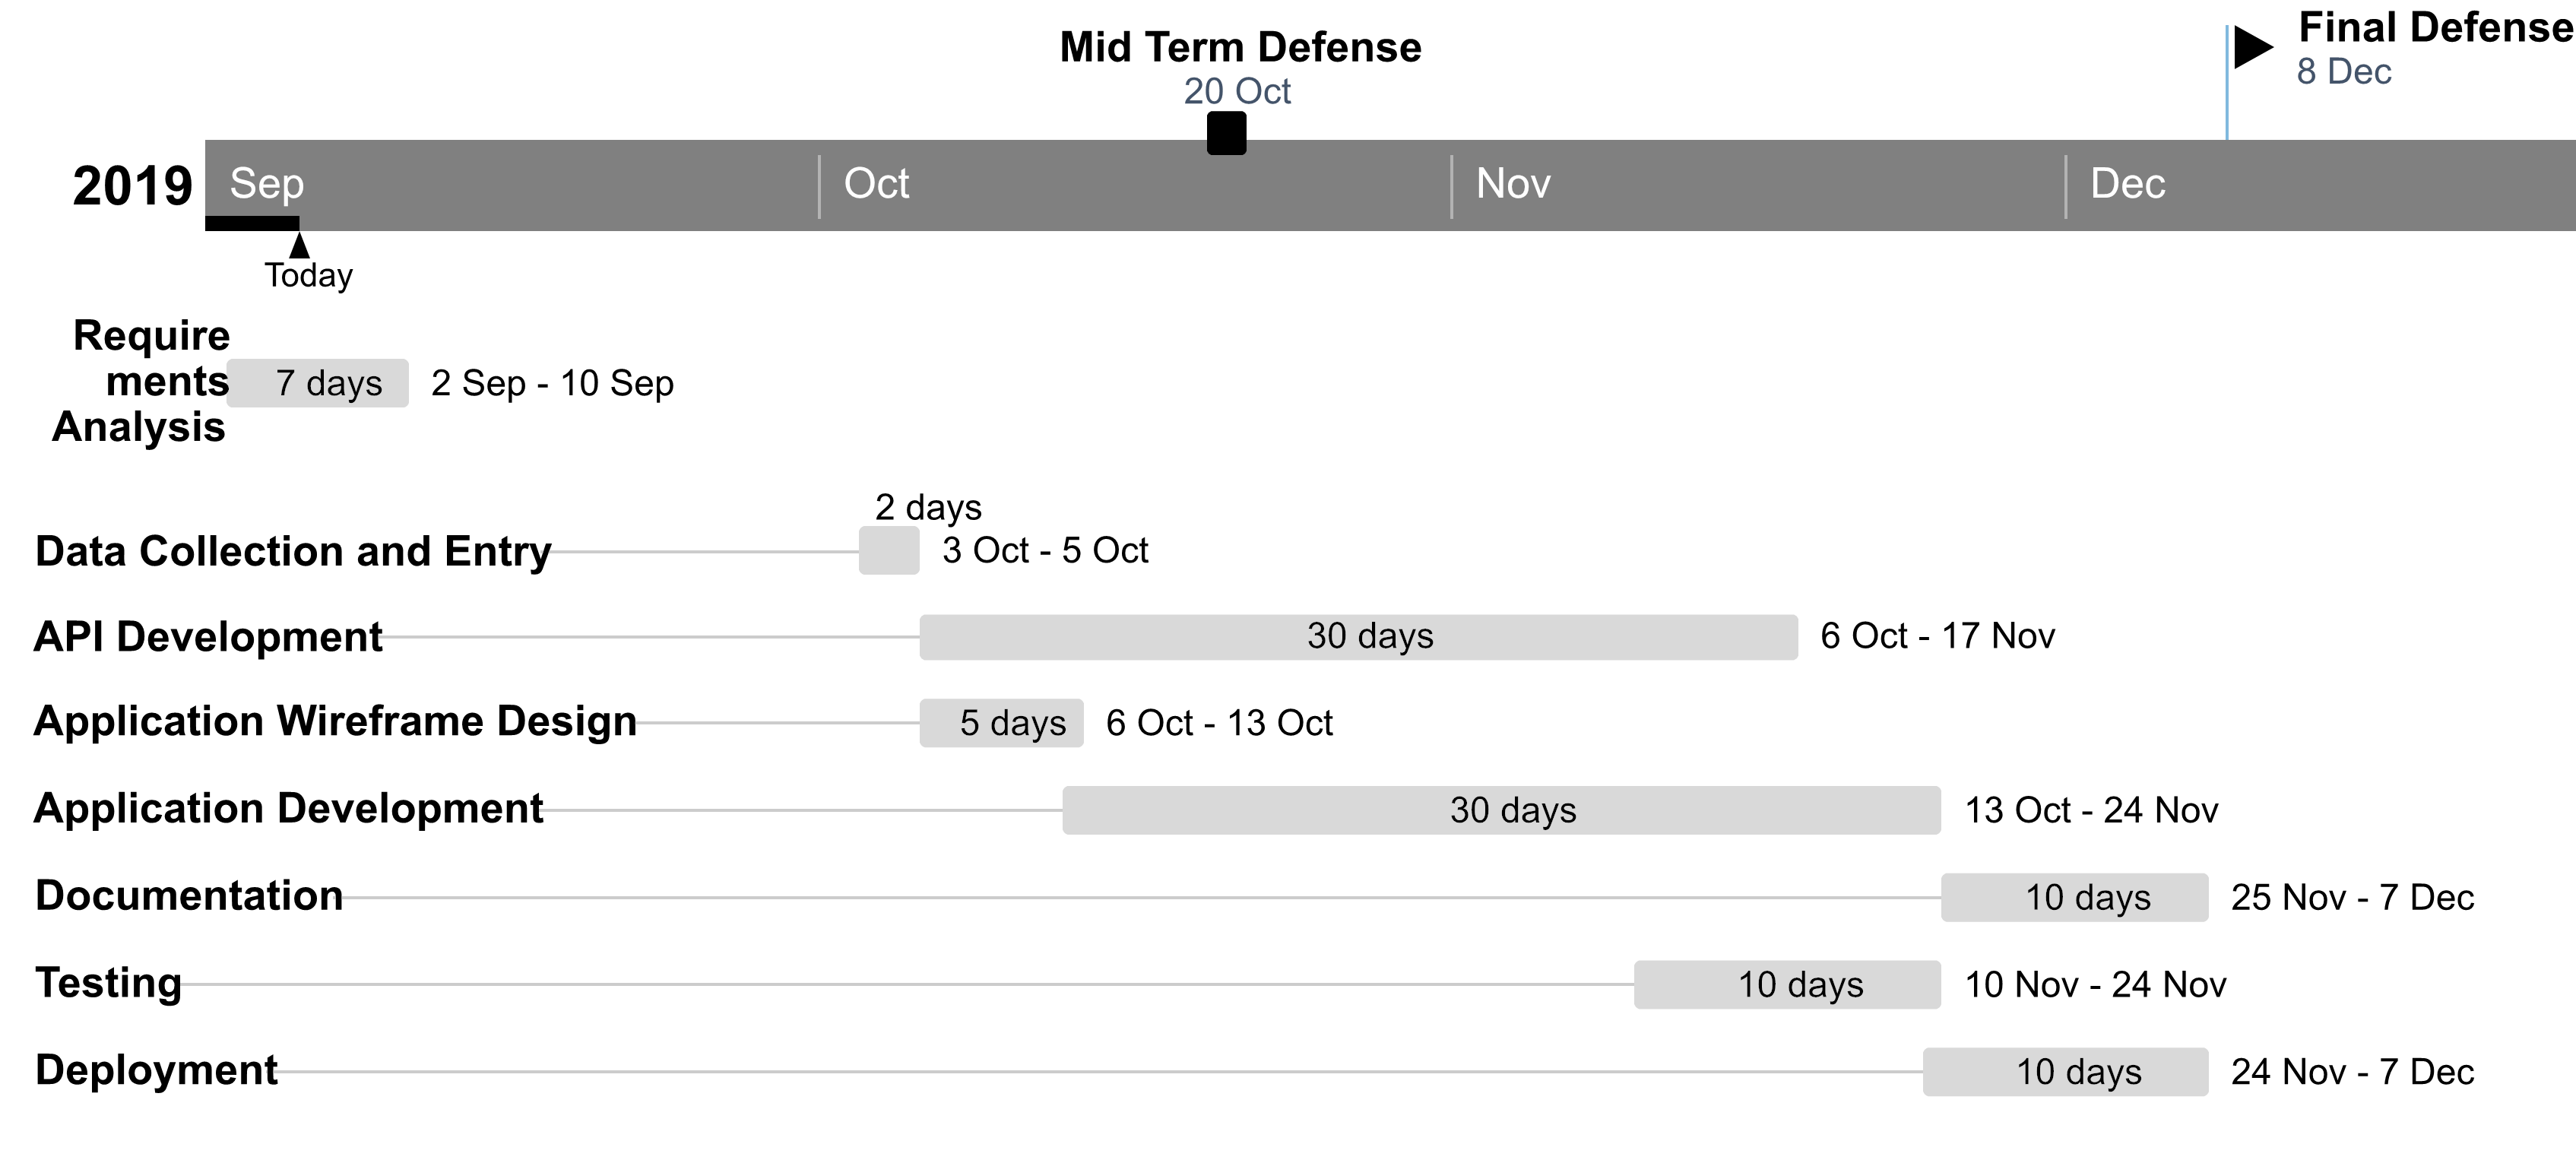
\includegraphics[width=\linewidth]{schedule}
	\centering
	\caption{Proposed project schedule}
	\label{fig:schedule}
\end{figure}



\break
\addcontentsline{toc}{section}{References}
\bibliography{references}
\bibliographystyle{ieeetran}

\end{document}